\documentclass{article}  
% Include all project wide packages here.
\usepackage{fullpage}
\usepackage{polyglossia}
\setmainlanguage{dutch}
\usepackage{csquotes}
\usepackage{graphicx}
\usepackage{epstopdf}
\usepackage{pdfpages}
\usepackage{caption}
\usepackage[list=true]{subcaption}
\usepackage{float}
%\usepackage{mathtools}
\usepackage{standalone}
\usepackage{import}
\usepackage{tocloft}
\usepackage{wrapfig}
\usepackage{authblk}
\usepackage{array}
\usepackage{booktabs}
\usepackage[toc,page,title,titletoc]{appendix}
\usepackage{xunicode}
\usepackage{amsmath}
\usepackage{fontspec}
\usepackage{unicode-math}
\usepackage[
    backend=bibtexu,
	texencoding=utf8,
bibencoding=utf8,
    style=ieee,
    sortlocale=nl_NL,
    language=auto
]{biblatex}
\usepackage{listings}
\newcommand{\includecode}[3][c]{\lstinputlisting[caption=#2, escapechar=, style=#1]{#3}}
\newcommand{\superscript}[1]{\ensuremath{^{\textrm{#1}}}}
\newcommand{\subscript}[1]{\ensuremath{_{\textrm{#1}}}}


\newcommand{\chapternumber}{\thechapter}
\renewcommand{\appendixname}{Bijlage}
\renewcommand{\appendixtocname}{Bijlagen}
\renewcommand{\appendixpagename}{Bijlagen}

\usepackage[hidelinks]{hyperref} %<--------ALTIJD ALS LAATSTE
  
\renewcommand{\familydefault}{\sfdefault}

\setmainfont[Ligatures=TeX]{Myriad Pro}
\setmathfont{Asana Math}
\setmonofont{Lucida Console}

\usepackage{titlesec, blindtext, color}
\definecolor{gray75}{gray}{0.75}
\newcommand{\hsp}{\hspace{20pt}}
\titleformat{\chapter}[hang]{\Huge\bfseries}{\chapternumber\hsp\textcolor{gray75}{|}\hsp}{0pt}{\Huge\bfseries}
\renewcommand{\familydefault}{\sfdefault}
\renewcommand{\arraystretch}{1.2}
\setlength\parindent{0pt}

%For code listings
\definecolor{black}{rgb}{0,0,0}
\definecolor{browntags}{rgb}{0.65,0.1,0.1}
\definecolor{bluestrings}{rgb}{0,0,1}
\definecolor{graycomments}{rgb}{0.4,0.4,0.4}
\definecolor{redkeywords}{rgb}{1,0,0}
\definecolor{bluekeywords}{rgb}{0.13,0.13,0.8}
\definecolor{greencomments}{rgb}{0,0.5,0}
\definecolor{redstrings}{rgb}{0.9,0,0}
\definecolor{purpleidentifiers}{rgb}{0.01,0,0.01}


\lstdefinestyle{csharp}{
language=[Sharp]C,
showspaces=false,
showtabs=false,
breaklines=true,
showstringspaces=false,
breakatwhitespace=true,
escapeinside={(*@}{@*)},
columns=fullflexible,
commentstyle=\color{greencomments},
keywordstyle=\color{bluekeywords}\bfseries,
stringstyle=\color{redstrings},
identifierstyle=\color{purpleidentifiers},
basicstyle=\ttfamily\small}

\lstdefinestyle{c}{
language=C,
showspaces=false,
showtabs=false,
breaklines=true,
showstringspaces=false,
breakatwhitespace=true,
escapeinside={(*@}{@*)},
columns=fullflexible,
commentstyle=\color{greencomments},
keywordstyle=\color{bluekeywords}\bfseries,
stringstyle=\color{bluestrings},
identifierstyle=\color{purpleidentifiers}
}

\lstdefinestyle{vhdl}{
language=VHDL,
showspaces=false,
showtabs=false,
breaklines=true,
showstringspaces=false,
breakatwhitespace=true,
escapeinside={(*@}{@*)},
columns=fullflexible,
commentstyle=\color{greencomments},
keywordstyle=\color{bluekeywords}\bfseries,
stringstyle=\color{redstrings},
identifierstyle=\color{purpleidentifiers}
}

\lstdefinestyle{xaml}{
language=XML,
showspaces=false,
showtabs=false,
breaklines=true,
showstringspaces=false,
breakatwhitespace=true,
escapeinside={(*@}{@*)},
columns=fullflexible,
commentstyle=\color{greencomments},
keywordstyle=\color{redkeywords},
stringstyle=\color{bluestrings},
tagstyle=\color{browntags},
morestring=[b]",
  morecomment=[s]{<?}{?>},
  morekeywords={xmlns,version,typex:AsyncRecords,x:Arguments,x:Boolean,x:Byte,x:Char,x:Class,x:ClassAttributes,x:ClassModifier,x:Code,x:ConnectionId,x:Decimal,x:Double,x:FactoryMethod,x:FieldModifier,x:Int16,x:Int32,x:Int64,x:Key,x:Members,x:Name,x:Object,x:Property,x:Shared,x:Single,x:String,x:Subclass,x:SynchronousMode,x:TimeSpan,x:TypeArguments,x:Uid,x:Uri,x:XData,Grid.Column,Grid.ColumnSpan,Click,ClipToBounds,Content,DropDownOpened,FontSize,Foreground,Header,Height,HorizontalAlignment,HorizontalContentAlignment,IsCancel,IsDefault,IsEnabled,IsSelected,Margin,MinHeight,MinWidth,Padding,SnapsToDevicePixels,Target,TextWrapping,Title,VerticalAlignment,VerticalContentAlignment,Width,WindowStartupLocation,Binding,Mode,OneWay,xmlns:x}
}

%defaults
\lstset{
basicstyle=\ttfamily\small,
extendedchars=false,
numbers=left,
numberstyle=\ttfamily\tiny,
stepnumber=1,
tabsize=4,
numbersep=5pt
}  

\author{
Robin Hes (4236815) \and Peter Stijnman (4215788) \and Xenia Wesdijk (4144074) \\

\textbf{In opdracht van:} \\
Erwin de Haan (4222814) \\
Tu Hoang (4203496) \\
}
\title{EPO3-1 - Opdracht 3: Moduleontwerp PWM generator}
\date{23 september 2013}
\begin{document}
\maketitle
\section{Samenvatting}
Dit document is een ontwerprapport over de moduleopdracht bij het project ``Maak een chip'' (EE2821). De gekozen module is een PWM-generator.
In dit rapport wordt beschreven hoe er aan de hand van een, door twee medestudenten, opgestelde lijst met specificaties tot een werkend ontwerp is gekomen.
In de inleiding (sectie \ref{sec:pwm-inl}) wordt de context van deze opdracht uiteengezet, vervolgens worden de opgestelde specificaties gegeven, zoals wij deze aangeleverd hebben gekregen (sectie \ref{sec:pwm-spec}), daarna het opgestelde ontwerp (sectie \ref{sec:pwm-ontw}) en tot slot de uitgewerkte implementatie met bebehorende validatie door middel van switch-level simulaties in Modelsim (sectie \ref{sec:pwm-impl}).

\tableofcontents

\section{Inleiding}
\label{sec:pwm-inl}
Het doel van deze opdracht is voornamelijk het oefenen met het maken van een ontwerp en implementatie voor een PWM-generator. Dit doen we aan de hand van een lijst vastgestelde specificaties met tenminste één parameter. In ons geval zijn het er twee: één hoofdparameter en één die daarvan afhankelijk is. Deze constructie is zo gekozen om te voorkomen dat de chip arithmetiek toe moet passen op de parameter voordat deze bruikbaar is. Ook helpt deze opdracht ons bij het ons verder eigen maken van het programma GoWithTheFlow.
Mogelijkerwijs hebben we voor onze eindopdracht ook nog een PWM-generator nodig, bijvoorbeeld als tijdssignaal met een lagere frequentie dan de clk. Mocht dit het geval zijn, dan is het mooi meegenomen dat we deze implementatie al gebouwd hebben.

\section{Specificatie voor PWM generator}
\label{sec:pwm-spec}
Wij hebben de volgende specificaties gekregen, waaraan onze implementatie voldoet:

\subimport{pwm_gen}{specificaties-pwm-gen.tex}

De initiële specificaties lieten nog wat onduidelijkheden over. Na enig overleg met de opdrachtgevers zijn de specificaties verduidelijkt en konden wij aan de slag met ons ontwerp.

\section{Ontwerp}
\label{sec:pwm-ontw}
Een PWM-generator is vrij gemakkelijk te implementeren met een counter, die klokpulsen telt, totdat de waarde van de divider is bereikt; en met een pulsgenerator, die aan de hand van de waarde van \textit{count} de uitgangswaarde \textit{pulse} hoog of laag maakt.
Schematisch kan dit worden weergegeven als in figuur \ref{fig:pwm-schem}. Er is gekozen om de puls eerst gedurende één klokpuls te bufferen, voor deze aan de uitgang verschijnt (de overgang van \textit{new\_pulse} naar \textit{pulse}), om overgangsverschijnselen te voorkomen. Wanneer \textit{enabled} laag is, blijft de counter tellen, maar is de uitgang altijd laag. Bij een reset worden zowel \textit{count} als \textit{pulse} op 0 gezet. Verder dient vermeld te worden dat het gehele proces, inclusief reset, synchroon verloopt.

\begin{figure}[H]
	\centering
	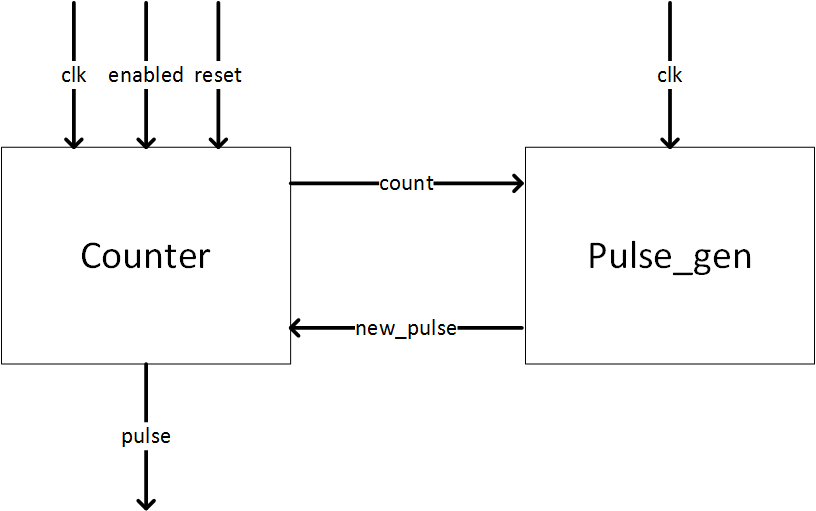
\includegraphics[width=0.6\textwidth]{resource/pwm_gen.png}
	\caption{Schematische weergave van de PWM-generator}
	\label{fig:pwm-schem}
\end{figure}

Er zou ervoor gekozen kunnen worden om de counter en de pulsgenerator modulair te implementeren. Dit zou kunnen resulteren in een kleiner chipoppervlak, omdat er dan meer controle kan worden uitgeoefend op de lay-out op switch-level. Omdat deze PWM-generator nog niet direct een doel heeft, hij maakt immers geen deel uit van een ander ontwerp en dus is er niet bepaald hoeveel bits deze PWM-generator dan zou moeten omvatten, hebben we er echter voor gekozen deze optimalisatiestap achterwege te laten. 
De schakeling bestaat dus uit slechts één ``blok''.

\section{Implementatie}
\label{sec:pwm-impl}
\footnotesize
Het onderstaande proces is doorlopen met drie verschillende bitsizes als parameter: 4-bits (divider: 15), 8-bits (divider: 255) en 16-bits (divider: 65535)

\normalsize
\subsection{Abstract}
\label{ssec:pwm-impl-abstr}
Het reeds beschreven ontwerp is vervolgens uitgewerkt in VHDL. Het resultaat hiervan, met bitsize 4, is te vinden in bijlage \ref{vhdl:pwm-gen} en de bijbehorende parameter package in bijlage \ref{vhdl:pwm-gen-pack}. Om de implementatie te testen hebben we deze gesimuleerd in Modelsim. Dit leverde het gewenste resultaat op, maar is slechts een indicatie voor de werkelijkheid.

\subsection{Synthese}
\label{ssec:pwm-impl-synth}
Ook synthese van de schakeling leverde geen problemen op, totdat de bitsize van de counter opgevoerd werd naar 16. Op dat moment begon de schakeling tijdens PWM-pulsen dips te vertonen van enkele nanoseconden. Hoogstwaarschijnlijk kwam dit doordat de hoeveelheid logica moest worden opgevoerd naar een niveau waar één klokperiode (100 ns) niet langer genoeg was om het uitgangssignaal zich in te laten stellen. Om dit op te lossen hebben we de eerder genoemde buffer bij de counter geïmplementeerd, waarna ook de simulatie op logisch niveau, met een 16-bits counter, correct werkte.
De gesynthetiseerde logische schakeling met een 4-bits counter is te zien in figuur \ref{fig:pwm-logic}.

\begin{figure}[H]
	\centering
	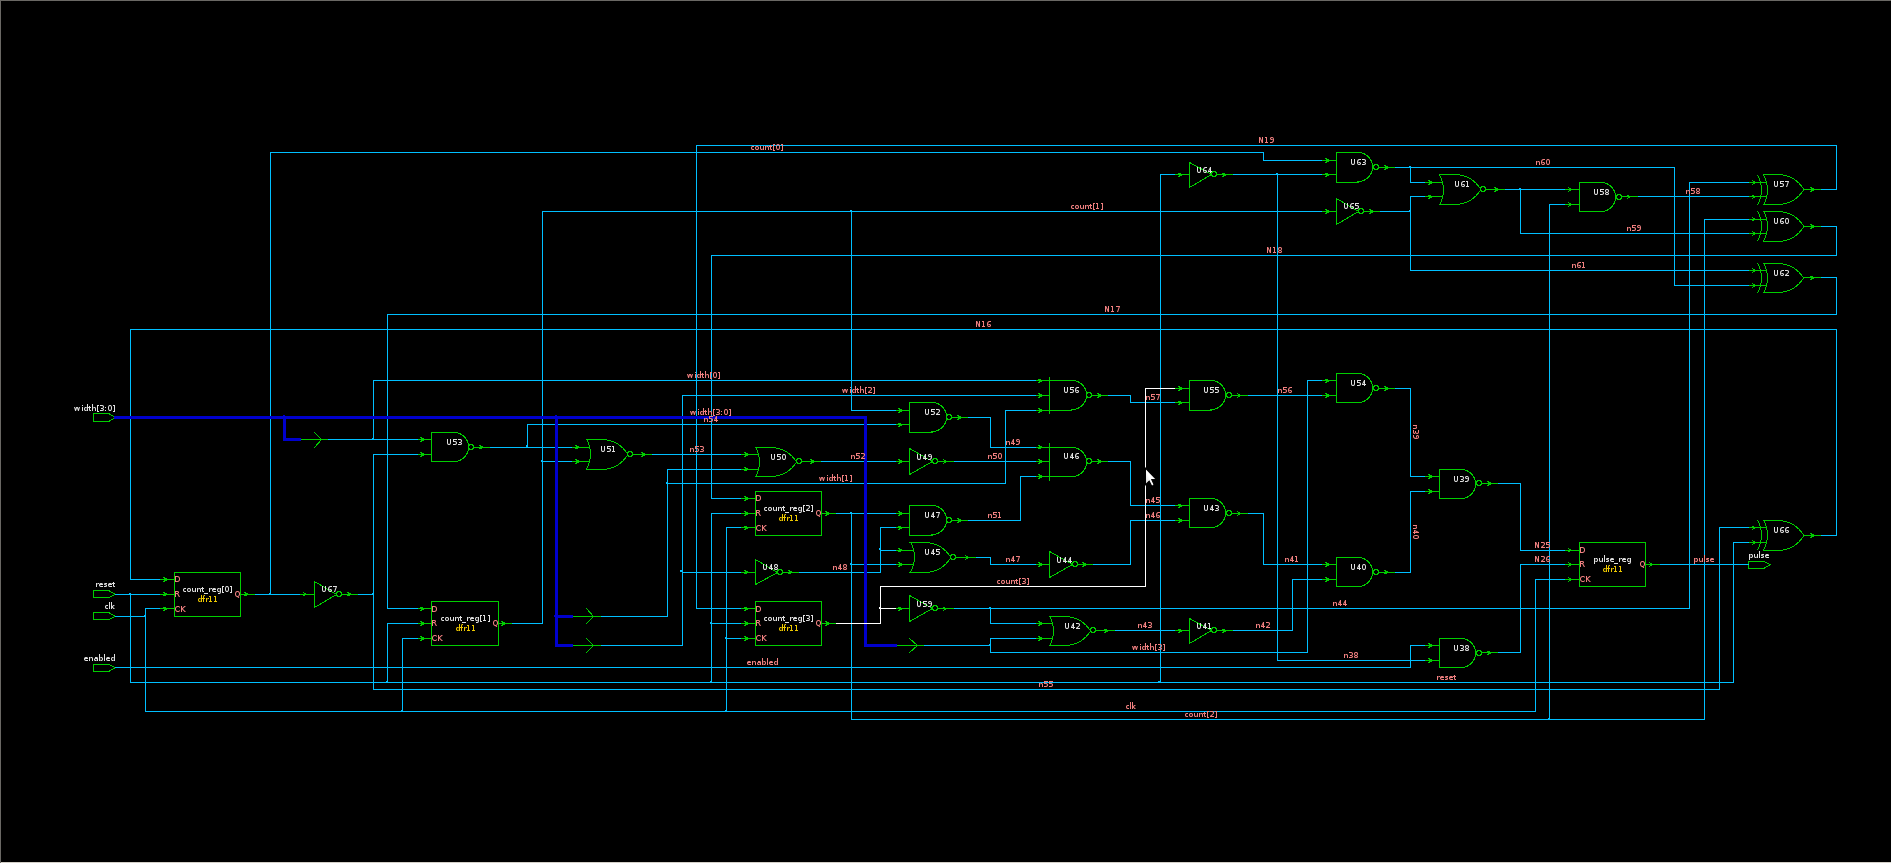
\includegraphics[width=\textwidth]{resource/pwm_gen_logic.png}
	\caption{De gesynthetiseerde logische schakeling met 4-bits counter. Merk de flip-flop (het buffer) voor de uitgang \textit{pulse} op}
	\label{fig:pwm-logic}
\end{figure}

\subsection{Lay-out}
\label{ssec:pwm-impl-layout}
Vervolgens was het zaak om een lay-out voor de schakeling te maken. Madonna was helaas niet in staat de rows zo te plaatsen dat Trout ze kon routen, dus we hebben zelf de rijen geplaatst om ze vervolgens met Trout te routen. De efficiëntie van dit proces lag voor elke bitsize rond de 50 \%. Het lijkt er dus op dat het vergroten van de bitsize, in ieder geval tot aan 16-bits, geen problemen oplevert tijdens het maken van een lay-out. Wanneer de PWM-generator gebruikt zal worden in het eindontwerp loont het pas de moeite hem te optimaliseren voor een bepaalde bitsize, bijvoorbeeld door het ontwerp modulair te maken en volledig handmatig te placen.
De gemaakte lay-out voor een 4-bits PWM-generator is te zien in figuur \ref{fig:pwm-layout}.

\begin{figure}[H]
	\centering
	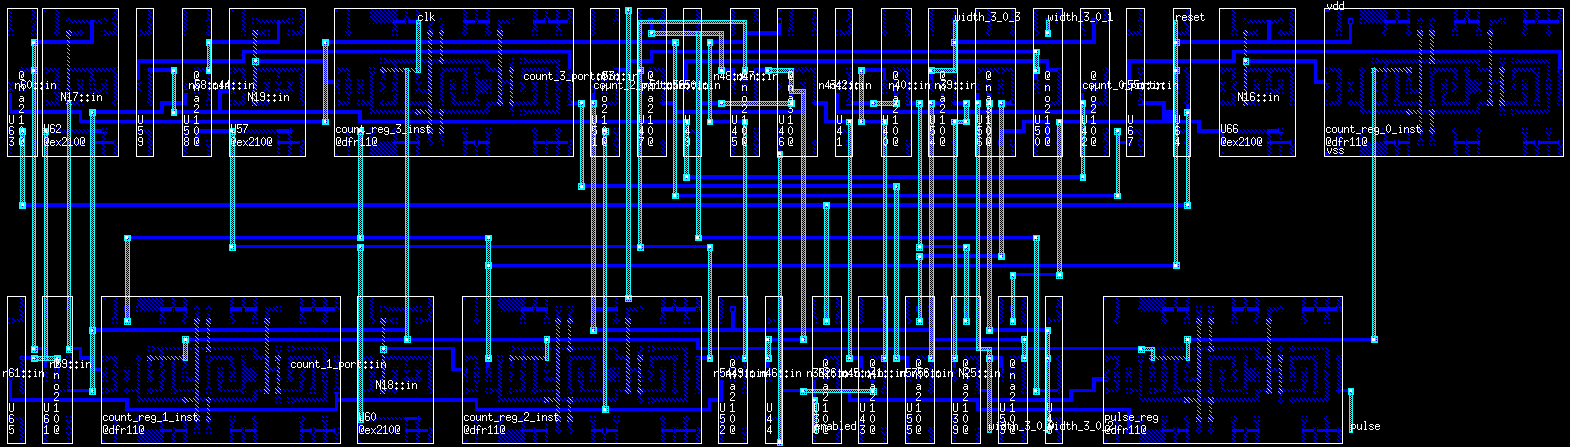
\includegraphics[width=\textwidth]{resource/pwm_gen_layout.png}
	\caption{De lay-out in Seadali voor een 4-bits PWM-generator}
	\label{fig:pwm-layout}
\end{figure}

\subsection{Switch-level simulatie}
\label{ssec:pwm-impl-switch}
Bovengenoemde lay-out hebben we voor elke geteste bitsize (4, 8 en 16) geëxtraheerd om ze vervolgens met Modelsim te simuleren. De testbench kan beschreven worden als de volgende sequentie: $width = 0$ (geen puls); $width = \frac{divider}{2}$ (lange puls); $width = divider$ (continu hoog): $width = 0$ (geen puls); $width = \frac{divider}{4}$ (korte puls). Bij de 16-bit simulatie geldt deze sequentie niet en werden andere (helaas willekeurige) pulslengten gebruikt, het gedrag is echter geverifiëerd tegen de gebruikte testbench.
De testbench (4-bit) is te vinden in bijlage \ref{vhdl:pwm-gen-tb}, de simulatieresultaten in de figuren \ref{sfig:pwm-sim-4bit}, \ref{sfig:pwm-sim-8bit} en \ref{sfig:pwm-sim-16bit}.

\begin{figure}[H]
	\centering
	\begin{subfigure}{\textwidth}
		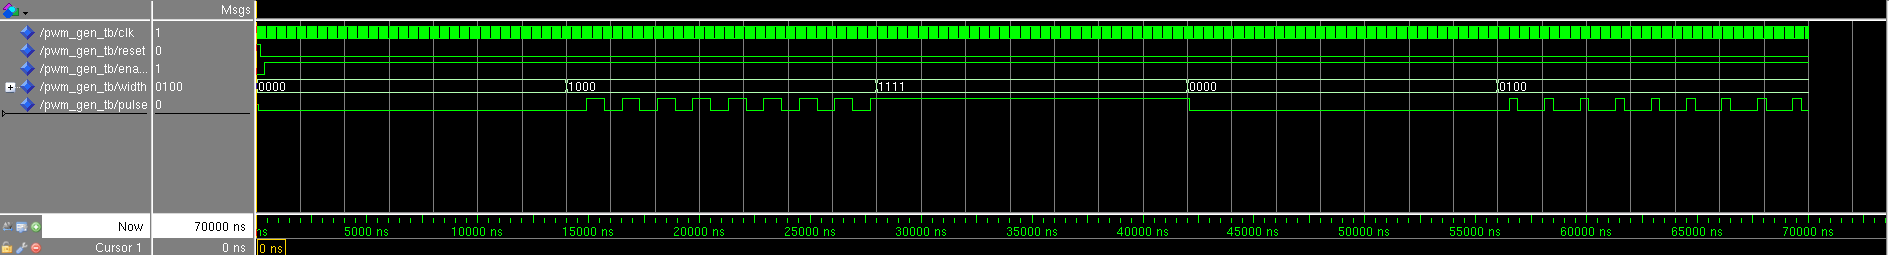
\includegraphics[width=\textwidth]{resource/pwm_gen_sim_4bit.png}
		\caption{Simulatieresultaat met 4-bit PWM-generator}
		\label{sfig:pwm-sim-4bit}
	\end{subfigure}
	\newline
	\begin{subfigure}{\textwidth}
		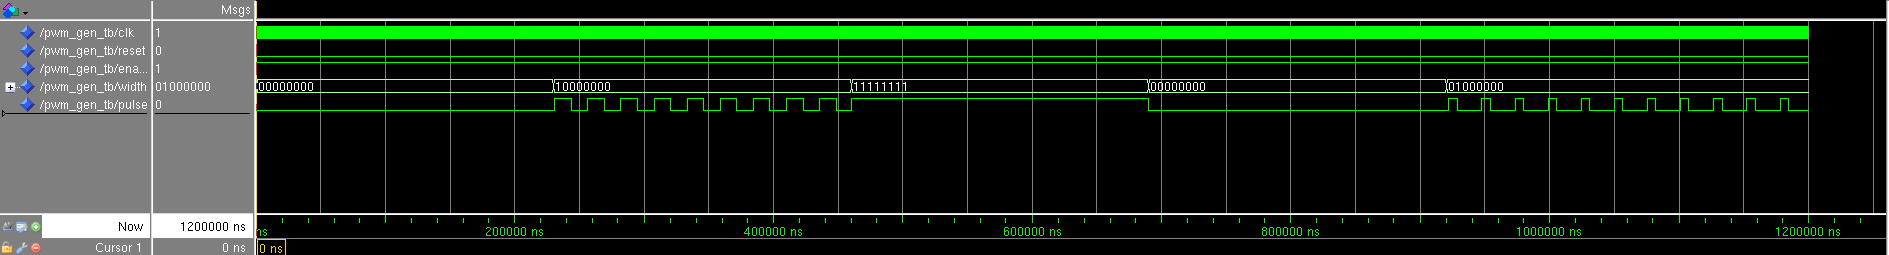
\includegraphics[width=\textwidth]{resource/pwm_gen_sim_8bit.png}
		\caption{Simulatieresultaat met 8-bit PWM-generator}
		\label{sfig:pwm-sim-8bit}
	\end{subfigure}
	\newline
	\begin{subfigure}{\textwidth}
		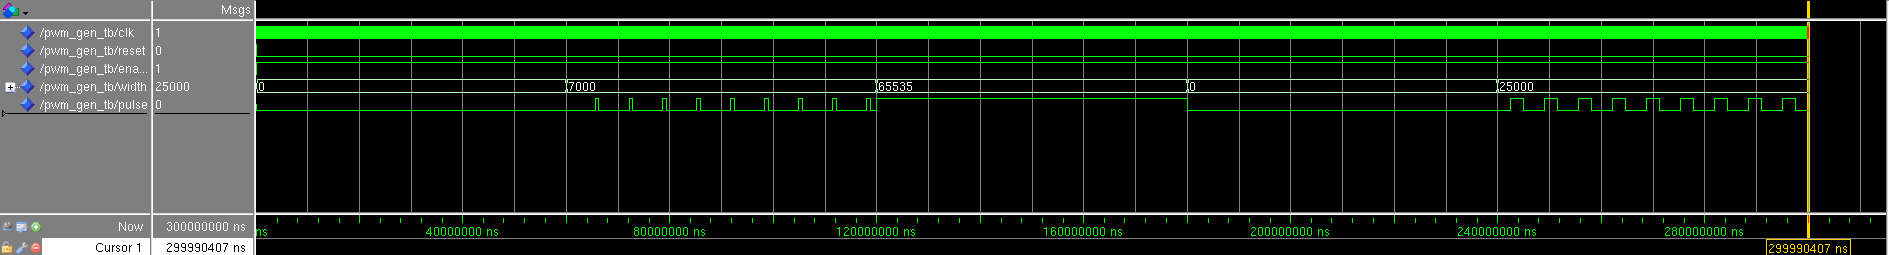
\includegraphics[width=\textwidth]{resource/pwm_gen_sim_16bit.png}
		\caption{Simulatieresultaat met 16-bit PWM-generator}
		\label{sfig:pwm-sim-16bit}
	\end{subfigure}
	\caption{Simulatieresultaten met extracted VHDL}
	\label{fig:pwm-sim}
\end{figure}

Vergeleken met de gebruikte testbenches leverden deze simulaties de verwachte resultaten en dus mag gesteld worden dat de implementatie voor iedere geteste bitsize correct functioneert.

\section{Conclusie}
\label{sec:pwm-conclusie}

\subsection{Vergelijking met specificatie}
\label{ssec:pwm-conclusie-spec-comp}
Het ontwerp is volledig volgens de specificatie gemaakt en ook de implementatie voldoet aan al de gestelde eisen en randvoorwaarden. Voor de simulaties is gebruikgemaakt van de hoogste klokfrequentie die binnen de specificaties mogelijk is, namelijk 100 mHz. Er mag vanuit gegaan worden dat lagere klokfrequenties dan ook geen problemen opleveren.
Al met al is het dus een geslaagd ontwerp.

\subsection{Verbeterpunten}
\label{ssec:pwm-conclusie-verb}
Zoals vermeld in sectie \ref{ssec:pwm-impl-layout} zou het mogelijk moeten zijn om de efficiëntie tijdens place \& route te verhogen zodat minder chipoppervlak wordt gebruikt. Wanneer de PWM-generator gebruikt gaat worden in het eindproduct is het tijd om optimalisaties te overwegen.

\section{Bijlagen}
\label{sec:pwm-bijlagen}

\subsection{VHDL parameter package (4-bit)}
\label{vhdl:pwm-gen-pack}
\includecode[VHDL]{parameter\_def\_pkg.vhd}{resource/parameter_def_pkg.vhd}

\subsection{VHDL PWM-generator (4-bit)}
\label{vhdl:pwm-gen}
\includecode[VHDL]{pwm\_gen.vhd}{resource/pwm_gen.vhd}
\includecode[VHDL]{pwm\_gen-behaviour.vhd}{resource/pwm_gen-behaviour.vhd}

\subsection{VHDL PWM-generator testbench (4-bit)}
\label{vhdl:pwm-gen-tb}
\includecode[VHDL]{pwm\_gen\_tb.vhd}{resource/pwm_gen_tb.vhd}
\includecode[VHDL]{pwm\_gen\_tb-behaviour.vhd}{resource/pwm_gen_tb-behaviour.vhd}


\end{document}
